\documentclass{standalone}
\usepackage{amsmath}
\usepackage{tikz}

\begin{document}
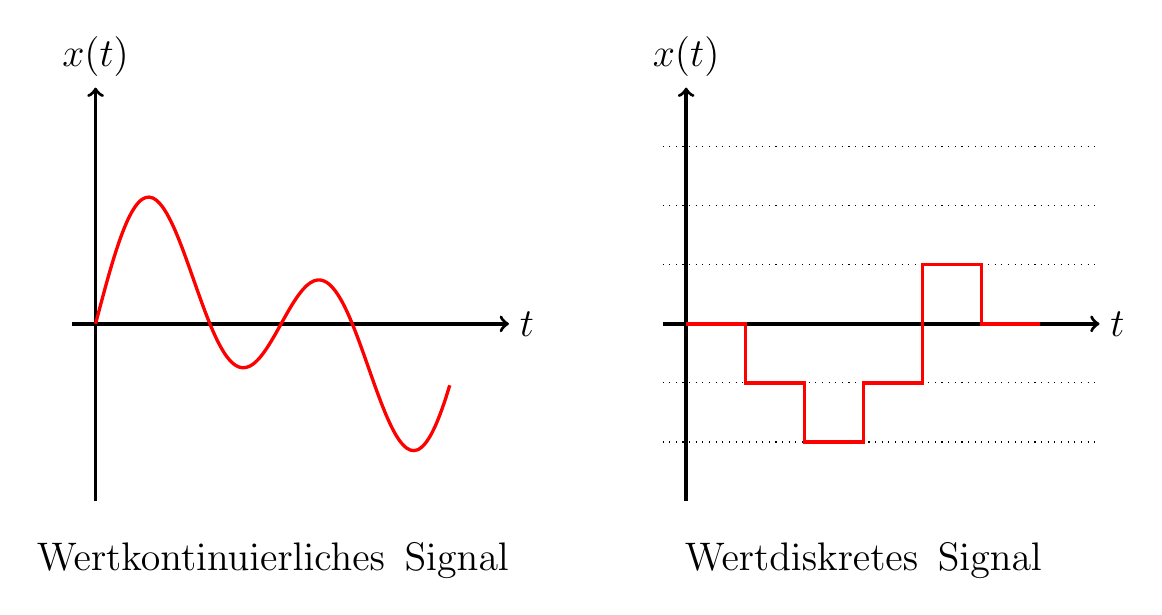
\begin{tikzpicture}[scale=1.5]

% Wertkontinuierliches Signal (links)
\begin{scope}
    \draw[->, very thick] (-0.2,0) -- (3.5,0) node[right] {\Large $t$};
    \draw[->, very thick] (0,-1.5) -- (0,2) node[above] {\Large $x(t)$};
    
    % Das kontinuierliche Signal
    \draw[red, very thick, domain=0:3, samples=100,smooth] 
        plot(\x,{0.5*sin(2*\x r) + 0.7*sin(4*\x r)});
        
    \node at (1.5,-2) {\text{\Large Wertkontinuierliches\, Signal}};
\end{scope}

% Wertdiskretes Signal (rechts)
\begin{scope}[xshift=5cm]
    \draw[->, very thick] (-0.2,0) -- (3.5,0) node[right] {\Large $t$};
    \draw[->, very thick] (0,-1.5) -- (0,2) node[above] {\Large $x(t)$};
    
    % Die horizontalen Linien für das Quantisierungsgitter
    \foreach \y in {-1,-0.5,0,0.5,1,1.5} {
        \draw[dotted] (-0.2,\y) -- (3.5,\y);
    }
    
    % Das diskrete Treppensignal (wertdiskret)
    \draw[very thick, red] (0, 0) -- (0.5, 0) -- (0.5, -0.5) -- (1, -0.5) -- (1, -1)
                 -- (1.5, -1) -- (1.5, -0.5) -- (2, -0.5) -- (2, 0.5) 
                 -- (2.5, 0.5) -- (2.5, 0) -- (3, 0);

    \node at (1.5,-2) {\Large\text{Wertdiskretes\, Signal}};
\end{scope}

\end{tikzpicture}
\end{document}
